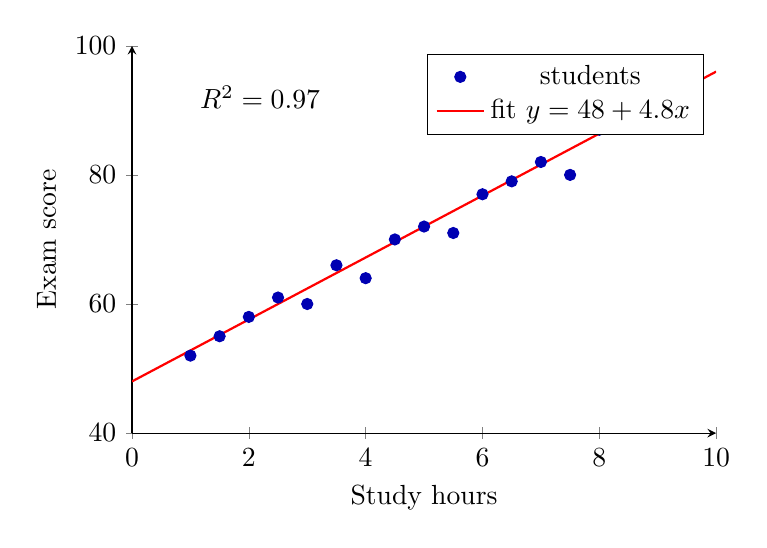
\begin{tikzpicture}
\begin{axis}[
    xlabel={Study hours},
    ylabel={Exam score},
    axis lines=left,
    xmin=0, xmax=10, ymin=40, ymax=100,
    width=9cm, height=6.5cm,
]
\addplot[only marks, mark=*, blue!70!black, mark size=2pt] coordinates {
  (1,52) (1.5,55) (2,58) (2.5,61) (3,60) (3.5,66) (4,64) (4.5,70) (5,72)
  (5.5,71) (6,77) (6.5,79) (7,82) (7.5,80) (8,87) (8.5,88) (9,91) (9.5,94)
};
\addplot[red, thick, domain=0:10] {48 + 4.8*x};
\addlegendentry{students}
\addlegendentry{fit $y = 48 + 4.8x$}
\node[anchor=west] at (axis cs:1,92) {$R^2 = 0.97$};
\end{axis}
\end{tikzpicture}
